\documentclass[ngerman]{scrreprt}
%

% 1.5-facher Zeilenabstand:
\usepackage[onehalfspacing]{setspace} 

\usepackage[utf8]{inputenc}
\usepackage[ngerman]{babel}
% Durchgehende Nummerierung von Abbildungen über
% Chapter hinaus
%\usepackage{chngcntr}
%\counterwithout{figure}{chapter}
%
% Kommentare mit \comment{}-Umgebung
\usepackage{verbatim}
%
\usepackage[%
    backend=biber,
    style=numeric,
    %style=alphabetic,
    %citestyle=alphabetic-verb,
    %citestyle=numeric
    %sorting=ynt    % Sortierung nach Name des Autors
    sorting=none    % Sortierung nach Auftreten
]{biblatex}
%\addbibresource{data/bibliography.bib}
\addbibresource{Bachelorarbeit.bib}

\usepackage{fancyvrb}
\usepackage{listings}

\lstset{literate=%
  {Ö}{{\"O}}1
  {Ä}{{\"A}}1
  {Ü}{{\"U}}1
  {ß}{{\ss}}2
  {ü}{{\"u}}1
  {ä}{{\"a}}1
  {ö}{{\"o}}1
}


\usepackage{minted}
\usepackage[german]{fancyref}
\usepackage{enumitem}
\usepackage{array}
\usepackage{graphicx}
\usepackage{multicol}
%\usepackage{pgf-umlsd}
%\usepackage[pict2e]{struktex}
\usepackage{tikz}
%\usetikzlibrary{arrows,shadows}
%\usepackage{csvsimple}
%\usepackage{pgfplots}
\usepackage{filecontents}
%\usepackage{../daten/tikz-uml}

% Anführungsstriche mit \enquote{}-Umgebung
\usepackage[autostyle]{csquotes} 

% =============================
\usepackage[colorinlistoftodos,prependcaption,textsize=tiny]{todonotes}

% Hyperlinks in PDF-Version des Dokumentes. Option sagt, dass keine roten Boxen erzeugt werden sollen.
\usepackage[pdfborder={0 0 0}]{hyperref} 

% Todo commands
% https://mirror.hmc.edu/ctan/macros/latex/contrib/todonotes/todonotes.pdf
\newcommand{\insertMore}[1]{\todo[inline, color=green!40]{#1 ergänzen}}
\newcommand{\insertRef}[1]{\todo[color=blue!40]{#1 (Referenz fehlt)}}
\newcommand{\importantTodo}[1]{\todo[color=red!40]{#1 (Wichtig!)}}

% Programmcode


\begin{comment}

\usepackage{geometry}
\geometry{
  left=2.5cm,
  right=2.5cm,
  top=2cm,
  bottom=2cm,
  bindingoffset=5mm
}

\end{comment}

\definecolor{lightgray}{rgb}{0.95, 0.95, 0.95}
\definecolor{darkgray}{rgb}{0.4, 0.4, 0.4}
%\definecolor{purple}{rgb}{0.65, 0.12, 0.82}
\definecolor{editorGray}{rgb}{0.95, 0.95, 0.95}
\definecolor{editorOcher}{rgb}{1, 0.5, 0} % #FF7F00 -> rgb(239, 169, 0)
\definecolor{editorGreen}{rgb}{0, 0.5, 0} % #007C00 -> rgb(0, 124, 0)
\definecolor{orange}{rgb}{1,0.45,0.13}		
\definecolor{olive}{rgb}{0.17,0.59,0.20}
\definecolor{brown}{rgb}{0.69,0.31,0.31}
\definecolor{purple}{rgb}{0.38,0.18,0.81}
\definecolor{lightblue}{rgb}{0.1,0.57,0.7}
\definecolor{lightred}{rgb}{1,0.4,0.5}
\usepackage{upquote}
% CSS
\lstdefinelanguage{CSS}{
  keywords={color,background-image:,margin,padding,font,weight,display,position,top,left,right,bottom,list,style,border,size,white,space,min,width, transition:, transform:, transition-property, transition-duration, transition-timing-function},	
  sensitive=true,
  morecomment=[l]{//},
  morecomment=[s]{/*}{*/},
  morestring=[b]',
  morestring=[b]",
  alsoletter={:},
  alsodigit={-}
}

% JavaScript
\lstdefinelanguage{JavaScript}{
  morekeywords={typeof, new, true, false, catch, function, return, null, catch, switch, var, if, in, while, do, else, case, break},
  morecomment=[s]{/*}{*/},
  morecomment=[l]//,
  morestring=[b]",
  morestring=[b]'
}

\lstdefinelanguage{HTML5}{
  language=html,
  sensitive=true,	
  alsoletter={<>=-},	
  morecomment=[s]{<!-}{-->},
  tag=[s],
  otherkeywords={
  % General
  >,
  % Standard tags
	<!DOCTYPE,
  </html, <html, <head, <title, </title, <style, </style, <link, </head, <meta, />,
	% body
	</body, <body,
	% Divs
	</div, <div, </div>, 
	% Paragraphs
	</p, <p, </p>,
	% scripts
	</script, <script,
  % More tags...
  <canvas, /canvas>, <svg, <rect, <animateTransform, </rect>, </svg>, <video, <source, <iframe, </iframe>, </video>, <image, </image>, <header, </header, <article, </article
  },
  ndkeywords={
  % General
  =,
  % HTML attributes
  charset=, src=, id=, width=, height=, style=, type=, rel=, href=,
  % SVG attributes
  fill=, attributeName=, begin=, dur=, from=, to=, poster=, controls=, x=, y=, repeatCount=, xlink:href=,
  % properties
  margin:, padding:, background-image:, border:, top:, left:, position:, width:, height:, margin-top:, margin-bottom:, font-size:, line-height:,
	% CSS3 properties
  transform:, -moz-transform:, -webkit-transform:,
  animation:, -webkit-animation:,
  transition:,  transition-duration:, transition-property:, transition-timing-function:,
  }
}

\lstdefinestyle{htmlcssjs} {%
  % General design
%  backgroundcolor=\color{editorGray},
  basicstyle={\footnotesize\ttfamily},   
  frame=b,
  % line-numbers
  xleftmargin={0.75cm},
  numbers=left,
  stepnumber=1,
  firstnumber=1,
  numberfirstline=true,	
  % Code design
  identifierstyle=\color{black},
  keywordstyle=\color{blue}\bfseries,
  ndkeywordstyle=\color{editorGreen}\bfseries,
  stringstyle=\color{editorOcher}\ttfamily,
  commentstyle=\color{brown}\ttfamily,
  % Code
  language=HTML5,
  alsolanguage=JavaScript,
  alsodigit={.:;},	
  tabsize=2,
  showtabs=false,
  showspaces=false,
  showstringspaces=false,
  extendedchars=true,
  breaklines=true,
  % German umlauts
  literate=%
  {Ö}{{\"O}}1
  {Ä}{{\"A}}1
  {Ü}{{\"U}}1
  {ß}{{\ss}}1
  {ü}{{\"u}}1
  {ä}{{\"a}}1
  {ö}{{\"o}}1
}
%
\lstdefinestyle{py} {%
language=python,
literate=%
*{0}{{{\color{lightred}0}}}1
{1}{{{\color{lightred}1}}}1
{2}{{{\color{lightred}2}}}1
{3}{{{\color{lightred}3}}}1
{4}{{{\color{lightred}4}}}1
{5}{{{\color{lightred}5}}}1
{6}{{{\color{lightred}6}}}1
{7}{{{\color{lightred}7}}}1
{8}{{{\color{lightred}8}}}1
{9}{{{\color{lightred}9}}}1,
basicstyle=\footnotesize\ttfamily, % Standardschrift
numbers=left,               % Ort der Zeilennummern
%numberstyle=\tiny,          % Stil der Zeilennummern
%stepnumber=2,               % Abstand zwischen den Zeilennummern
numbersep=5pt,              % Abstand der Nummern zum Text
tabsize=4,                  % Groesse von Tabs
extendedchars=true,         %
breaklines=true,            % Zeilen werden Umgebrochen
keywordstyle=\color{blue}\bfseries,
frame=b,
commentstyle=\color{brown}\itshape,
stringstyle=\color{editorOcher}\ttfamily, % Farbe der String
showspaces=false,           % Leerzeichen anzeigen ?
showtabs=false,             % Tabs anzeigen ?
xleftmargin=17pt,
framexleftmargin=17pt,
framexrightmargin=5pt,
framexbottommargin=4pt,
%backgroundcolor=\color{lightgray},
showstringspaces=false,      % Leerzeichen in Strings anzeigen ?
}%
%
\lstdefinelanguage{java}{%
  % Basic settings
  basicstyle=\smaller\ttfamily,
  tabsize=4,
  %frame=single,
  showstringspaces=false,
  mathescape=true,
  breaklines=true,
  numbers=left,
  % Keywords, strings, and comments
  keywords={%
    abstract, continue, for, new, switch, assert, default, goto, package,
    synchronized, boolean, do, if, private, this, break, double, implements,
    protected, throw, byte, else, import, public, throws, case, enum,
    instanceof, return, transient, catch, extends, int, short, try, char,
    final, interface, static, void, class, finally, long, strictfp, volatile,
    const, float, native, super, while
  },
  keywords=[2]{%
  },
  morestring=[b]",
  morestring=[b]',
  morecomment=[l]{//},
  morecomment=[s]{/*}{*/},
  % Colors and style
  %backgroundcolor=\color{BackgroundYellow},
  keywordstyle=\color{blue},
  keywordstyle=[2]\color{DarkOrchid},
  commentstyle=\color{ForestGreen},
  stringstyle=\color{Red},
  numberstyle=\color{SolarizedGrey}
}

\begin{document}

% Title
%
%
%
%
\begin{titlepage}
    \begin{tikzpicture}[remember picture,overlay]
		\node[anchor=north west,inner sep=0pt] at (current page.north west)
		{
\includegraphics[height=4cm]{data/bilder/fh-aachen.png}};
	\end{tikzpicture}
	\begin{flushright}
		\textbf{\Large Multimediale Unterstützung in der Medizinprodukteaufbereitung mittels Smartglasses}
		\linebreak
		\linebreak
		\textbf{\Large Bachelorarbeit}
		\linebreak
		\linebreak
		%\textsc{Werkzeugmaschinenlabor der RWTH Aachen\linebreak
		%	\linebreak Steinbachstraße 25\linebreak
		%	52074 Aachen\linebreak
		%	}
	\end{flushright}
	\vfill
	\begin{tabular*}{\linewidth}{ll}
	    \multicolumn{2}{l}{\textsc{Fachhochschule Aachen, Campus Jülich}}\\
		Fachbereich: & Medizintechnik und Technomathematik\\
		Studiengang: & Scientific Programming\\
		Student: & Martin Leonard Haufs\\ 
		Matrikelnummer: & 4015814
	\end{tabular*}
	\vfill	
	\centering\large Aachen, \dateOfSubmission % \today
\end{titlepage}

\setcounter{page}{1} 
\pagenumbering{roman}
\chapter*{Persönliche Erklärung}
%\flushleft
\begin{flushleft}
Diese Arbeit ist von mir selbstständig angefertigt und verfasst. 
Es sind keine anderen als die angegebenen Quellen und Hilfsmittel benutzt worden.
\linebreak
\linebreak
    %Aachen, den \today\linebreak	
    Name: \authorOfWork
    \linebreak 
    Aachen, den \dateOfSubmission%\today
    \linebreak	
    \linebreak
    Unterschrift: \underline{\hspace{5cm}}
    	
    \vspace{2.0cm}
    Diese Arbeit wurde betreut von: \linebreak
    
    \begin{tabular*}{\linewidth}{ll}
    	1. Prüfer: & \erstpruefer\\
    	2. Prüfer: & \zweitpruefer
    \end{tabular*}

\end{flushleft}


\tableofcontents

\begin{comment}
%
\begin{abstract}
	Hier steht die Zusammenfassung.
\end{abstract}
%
\end{comment}

\pagenumbering{arabic}

\setcounter{page}{1} 
%%
%
%
% - - - - - Einleitung - - - - - - - - 
%
%
%
\chapter{Einleitung}
\label{ch:Einleitung}
% 2 Seiten
Augmented Reality-Geräte gehören laut einer Analyse von Gartner zu den Top 10 Technologien für das Jahr 2018 \cite{Panetta2017a}. Es wird ein fundamentaler Wechsel in der Art und Weise erwartet, wie Nutzer mit der \emph{digitalen Welt} interagieren. 

Ebenso wie Augmented Reality gehören die sogenannten \emph{wearables} (am Körper getragene Computer) zu den Geräten mit den höchsten Erwartungen aus dem Jahre 2015 \cite{Levy2015}. Neben Smartwatches, die sich im privaten Bereich bereits durchgesetzt haben, werden Datenbrillen (Smart Glasses, Data Glasses, Head Mounted Displays (HMD), Head-Up Displays (HUD) oder auch Head Worn Displays \cite{Zobel2016}) neben dem privaten- auch im beruflichen Umfeld eingesetzt. Smartglasses sind eine der am intensivsten und vielversprechendsten diskutierten Technologien im professionellen Umfeld \cite{Hein2016}.

Die Mobilität von Computern nahm mit der Erfindung von Smartphones rasant zu. \emph{Wearable Technologies}, also am Körper getragene Computer beschleunigen diesen Effekt weiter. Computer gehören damit zum allgegenwärtigen Bestandteil des Lebens vieler Anwender und begleiten Nutzer den gesamten (Berufs-) Alltag hinweg. Wearables stellen eine völlig neuartige Schnittstelle zwischen Mensch und Computer dar \cite[S.~25f]{Schwenke2016}. Bei der Veröffentlichung kürte die Zeitschrift Time-Magazinne die Erfindung Google Glass als eine der \enquote{Best Inventions of the Year} \cite{Bilton2015}.

Smartglasses sind Brillen, die es ermöglichen, digitale Informationen direkt im realen Umfeld anzuzeigen. So haben Nutzer von Smartglasses die Informationen immer im Blickfeld, ohne auf ein Gerät wie ein Smartphone schauen zu müssen \cite{Due2014Glasses}.

Diese Interaktion mittels Augmented Reality-Wearables wie Smartglasses wird im beruflichen Umfeld bereits erfolgreich im Bereich der Logistikunternehmen eingesetzt \cite{Plutz}.
Ebenso werden sie in Museen als interaktiver Guide verwendet \cite{Hein2016}. 
Wearables bieten hier die Möglichkeit, im Arbeitsalltag in dem beispielsweise die Hände frei sein müssen, kontextbezogene Informationen bereitzustellen und so die Arbeit zu erleichtern \cite{Zobel2016}. Smartglasses ermöglichen es, kontextsensitive Informationen darzustellen und Objekte zu erkennen und zu klassifizieren.
%
\note{Überleitung zu ZSVA}
%

Operationen werden im heutigen Gesundheitswesen immer wichtiger. Für Operationen werden chirurgische Instrumente benötigt, die steril gehalten werden, sogenannte Sterilgüter.
Medizinische Instrumente in Krankenhäusern werden nicht nur immer kleiner, sondern auch immer teurer, sodass eine Wiederverwendung elementar wichtig ist. Dies geschieht durch sogenannte Sterilisation der Geräte, die in der Regel in der Medizinprodukteaufbereitung, die Teil der Zentralen Sterilgutversorgungsabteilung (ZSVA) von Krankenhäusern ist. In der ZSVA werden medizinische Geräte gereinigt, desinfiziert und sterilisiert und somit unter strengen rechtlichen und hygienischen Vorgaben wiederaufbereitet. 

Wie wichtig eine gut funktionierende Sterilgutversorgung ist zeigen Problemfälle wie im Uniklinikum Mannheim \cite{Brandt2015} aus dem Jahr 2015 oder im Klinikum Fulda im Jahr 2012 \cite{HygieneFuldar2012}, bei denen ein millionenschwerer Schaden durch mangelhaft sterilisierte chirurgische Instrumente entstanden ist. Eine gut funktionierende Sterilgutversorgung stellt also ein Kernthema der Patientensicherheit dar und ist gleichzeitig mit enormen Kostendruck verbunden, da es immer mehr zu Personaleinsparungen. Die ZSVA steht ebenfalls unter enormem Druck, da bedingt durch den hohen Preis die Anzahl der Geräte und chirurgischen Instrumente möglichst klein gehalten werden muss. Chirurgische Instrumente werden zudem immer komplexer und somit die Anforderungen an die Mitarbeiterinnen und Mitarbeiter der ZSVA immer höher. Durch die hohe Komplexität der Geräte sind oft nur einzelne Angestellte in der Lage, besonders komplizierte Instrumente aufzubereiten, was den Personalmangel nochmals erhöht.

Ziel einer technischen Unterstützung innerhalb der ZSVA ist, die Arbeit der Angestellten zu erleichtern und möglichst viele Personen in die Lage zu versetzen, bislang unbekannte Instrumente aufzuarbeiten.

Es wird immer wichtiger, die Angestellten der ZSVA auch mittels technischer Hilfsmittel zu unterstützen. Die Unterstützung mittels Augmented Reality über Smartglasses kann möglicherweise ein gutes Mittel sein, um im Feld der hoch infektiösen und steril gehaltenen Atmosphäre der Medizinprodukteaufbereitung eingesetzt zu werden. Die Brillen ermöglichen hier eine freihändige Bedienung und Bereitstellung von Informationen. Angestellte der ZSVA können nicht immer jeden Schritt der Sterilisation von über tausend verschiedenen Instrumenten kennen und benötigen daher Unterstützung. Es können mittels der Datenbrillen auf jedes medizinische Instrument angepasste Informationen dargestellt werden. 

Im Rahmen dieser Arbeit wird der Einsatz von Smartglasses in der ZSVA analysiert, die mögliche Unterstützung mittels multimedialer Anwendungen erörtert und mittels Experteninterviews evaluiert. 
%\chapter{Entwicklungsansätze mobiler Applikationen}
\label{chap:entwicklungsansaetze}
% Ansatz: Summe ca. 4 Seiten
%
% weitere Infos:
% http://www.uptopcorp.com/post/mobile-app-development-native-vs-hybrid-vs-mobile-websites
%
Im laufe der letzten Jahre haben sich verschiedene grundsätzliche Ansätze für die Entwicklung mobiler Applikationen etabliert. Bei der Wahl eines dieser Ansätze müssen verschiedene Anforderungen an die mobile Applikation betrachtet werden. Zunächst muss entschieden werden, welches Betriebssystem die App unterstützen soll. Dabei haben sich im laufe der letzten Jahre die Betriebssysteme iOS und Android durchgesetzt. Im dritten Quartal 2016 hatte iOS einen weltweiten Marktanteil von 12.1~\% und Android einen Marktanteil von 87.5~\% \cite{strategyAnalyticsMarktanteile}. Da die beiden Betriebssysteme somit einen gemeinsamen weltweiten Marktanteil von 99,6~\%  bilden, spielen die weiteren Systeme Windows Phone und Blackberry OS nur eine sehr untergeordnete Rolle.

Eines der Ziele einer mobilen Applikation ist es, eine für die Plattform typische Benutzererfahrung zu schaffen und keine großen Irritationen zu verursachen. Dies muss natürlich bei der Umsetzung beachtet werden \cite{FrancisHybridApp}.

Zur Entwicklung mobiler Applikationen gibt es grundsätzlich drei verschiedene Ansätze, die im Folgenden beschrieben und verglichen werden.
\begin{comment}
    
    Zur Entwicklung mobiler Applikationen gibt es grundsätzlich drei verschiedene Ansätze, die sich folgendermaßen charakterisieren lassen:
    \begin{itemize}
        \item Native Entwicklung der Applikation in der Programmiersprache, die ursprünglich für die Entwicklung auf dieser Plattform vorgesehen war
        \item Systemübergreifende Entwicklung mittels einer Web-Applikation
        \item Systemübergreifende Entwicklung mittels hybrider Frameworks
    \end{itemize}

\end{comment}
%
% --------------------------------------------------------------------------------------------
%
\section{Native Applikationen}
\label{sec:nativeApplikationen}
%
Unter nativer Anwendungsentwicklung wird die direkte Entwicklung für eine Plattform in der jeweiligen ursprünglichen Programmiersprache verstanden. Bei iOS ist die native Programmiersprache Objective-C bzw. zunehmend Swift \cite{appleDokuSwift}. Für Android wird nativ in Java programmiert \cite{googleAndroidDoku}. Google hat ein Framework namens \emph{Android NDK} veröffentlicht, mit dem es möglich ist, Teile einer Android App in einer anderen nativen Programmiersprache (C oder C++) zu entwickeln und in ein in Java entwickeltes Projekt einzubinden \cite{googleAndroidNDKDoku}. In ähnlichem Maße lassen sich in ein natives in Objective~C entwickeltes iOS-Projekt C++-Projekte einbinden \cite{appleDokuCppObjectiveC}. So ist es zumindest zum Teil möglich eine gemeinsame Codebasis (z.B. bei Datenmodellen) zwischen Android- und iOS-Projekten zu realisieren.
Ein großer Vorteil nativer Applikationen ist die hohe Performanz. Native Apps sind für ein bestimmtes Betriebssystem optimiert und daher für komplexe und rechenintensive Anwendungen sehr gut geeignet. Objective-C ist zudem als Erweiterung von C eine sehr maschinennahe Sprache \cite{appleObjectiveC}. 

Da iOS und Android als die beiden Hauptplattformen für mobile Applikationen zwei verschiedene native Programmiersprachen haben, müssen bei einem nativen Entwicklungsansatz auch größtenteils zwei getrennte Anwendungen entwickelt werden. Dies führt zu einem großen Mehraufwand in der Softwareentwicklung.

Neben der nativen Programmiersprache liefern die Plattformen auch hauseigene Entwicklungswerkzeuge. Für die iOS-Plattform gibt es die Entwicklungsumgebung Xcode, für Android wird das Android Studio bereitgestellt. Neben der nativen Programmiersprache spielen die Frameworks und Programmierschnittstellen, die APIs (\enquote{Application Programming Interface}) eine wichtige Rolle, da diese es erlauben, Zugriff auf die Hardwarefunktionalitäten des Gerätes zu nehmen. So kann mit wenig Aufwand Zugriff auf Kamera, GPS-Modul oder die verschiedenen Sensoren des mobilen Endgerätes zugegriffen werden. Zudem kann je nach System Zugriff auf die geschützten Daten des Gerätes wie Kalender oder Adressbuch des Nutzers genommen werden. 

Nativ entwickelte Apps lassen sich im jeweiligen App Store veröffentlichen und vertreiben. Zudem ermöglicht der App Store, Updates der Software veröffentlichen zu können. Apple unterzieht dabei jede App einem Review-Prozess. Um enge Qualitätsstandards zu gewährleisten lässt Apple dabei keine Apps im App Store zu, die beispielsweise plötzliche Abstürze, elementare Verstöße gegen die User Interface-Guidelines von Apple, kaum reale Funktionalität und damit keinen Mehrwert für den Nutzer oder inhaltliche Bedenken wie Verletzung gegen Jugendschutzvorgaben haben \cite{appleReview}. Zur Veröffentlichung im App Store ist eine Mitgliedschaft im Entwicklerportal nötig, die bei Apple 99,-~US-Dollar pro Jahr kostet. 
%
\subsection{Vorteile}
%
Aufgrund der Veröffentlichungsmöglichkeit in App Stores wird Entwicklern eine direkte Vertriebsmöglichkeit der eigenen Software geboten. Im Zuge der Qualitätskontrollen im App Store werden Applikationen mit schwerwiegenden Mängeln aussortiert und Anwendern ein gewisser Qualitätsanspruch für die im App Store angebotene Software garantiert.

Die nativen Frameworks schaffen eine plattformspezifische Nutzungserfahrung, die von reinen Webseiten oftmals nicht erreicht werden kann. Sie liefern dem Nutzer zudem die Möglichkeit auf Bereiche der mobilen Plattform oder Sensoren der Hardware zuzugreifen, auf die Web-Applikationen keinen Zugriff haben.

Da native Programme die volle Hardwareleistung des Gerätes nutzen können, ermöglichen diese weit rechenintensivere Anwendungen. So können 3D-Spiele oder Simulationen berechnet werden, die eine gute Ausnutzung der Hardwareperformance benötigen.
%
\subsection{Nachteile}
%
Bei nativer Softwareentwicklung muss für jede Plattform eine eigene Anwendung programmiert werden, was die Entwicklungskosten massiv erhöht. Da jede Plattform eigene Frameworks verwendet, die sich zum Teil gravierend in ihrer Funktionsweise unterscheiden, ist es für Anbieter mehrerer getrennt entwickelter Apps nur sehr schwer eine gleichwertige Benutzererfahrung aller Systeme zu ermöglichen. So kommt es vor, dass manche Funktionen nicht auf allen Plattformen zur Verfügung stehen.

Bei einer Aktualisierung der App muss stets ein Update über den App Store erfolgen, welche nur durch den Nutzer initialisiert werden können. Es ist also nicht zwingend sichergestellt, dass immer die aktuelle Version auf dem Gerät des Nutzers installiert ist.

Die Entwicklung nativer iOS Apps ist zudem mit dem Nachteil verbunden, dass diese nur auf Macs möglich ist, da nur hier der Code kompiliert werden kann.
%
% --------------------------------------------------------------------------------------------
%
\section{Mobile Web-Applikationen}
\label{mobileWebApplikationen}
%
Unter einer mobilen Web-Applikation wird eine Applikation verstanden, die ausschließlich im Browser des Smartphones ausgeführt wird. Die Anwendung wird dabei mit allen benötigten Daten wie HTML-Dateien, CSS-Stylesheets oder Bildern von einem Webserver geladen und mittels HTTP-Protokoll an den Client übertragen. Im Gegensatz zu statischen Websites sind Webapplikationen dynamisch und erlauben eine Interaktion des Nutzers mit der Webseite. Ermöglicht wird dies durch den Einsatz von Skriptsprachen wie JavaScript. 

Mobile Webapplikationen sind an die Anforderungen einer mobilen Plattform angepasst und opimiert. So ermöglicht der Einsatz von \emph{Responsive Webdesign}, dass sich das Erscheinungsbild (Struktur und das Styling) einer Webseite dynamisch an die Bildschirmgröße, das verwendete Betriebssystem, die verwendete Auflösung und die Ausrichtung des Gerätes anpasst. Zudem sind Eingaben auf Events wie \enquote{Touch}, \enquote{Swipe} oder \enquote{Pinch} optimiert. Im Idealfall wird das Design (CSS-Bibliotheken) und das Verhalten der dynamischen Website soweit angepasst, dass die Webseite kaum von einer nativen Applikation unterschieden werden kann. 

Mobile Web-Applikationen unterliegen den Beschränkungen des Sandbox-Designs der Webbrowser. Unter Sandboxing wird ein Sicherheitsmechanismus verstanden, bei dem einzelne Programme durch Isolation in einer geschützten Umgebung ausgeführt werden und der Zugriff auf Speicherbereiche außerhalb des eigenen Prozesses eingeschränkt wird. Um das System vor potentiell gefährlichen Angriffen durch eine Webseite zu schützen werden Webseiten auf mobilen Plattformen in Sandbox-Prozessen ausgeführt, die nur einen eingeschränkten Zugriff auf die Daten des Nutzers und die Hardwarefunktionalitäten des Gerätes haben. 

Neben der Möglichkeit die Webseite über den Browser aufzurufen bietet iOS zusätzlich die Möglichkeit, ein Lesezeichen der Web-App auf dem Startbildschirm zu hinterlegen. So entsteht verstärkt der Eindruck einer wirklichen App, obwohl in Wirklichkeit nur ein Browserfenster in Vollbildmodus geöffnet wird \cite{safariRef}.
%
\subsection{Vorteile}
%
Durch eine völlig plattformunabhängige Entwicklung kann derselbe Code auf allen Plattformen ausgeliefert werden. Somit werden mit vergleichsweise geringerem Entwicklungsaufwand als bei nativer Entwicklung mehr Nutzer erreicht werden. Zudem kann Code aus Desktop-Webanwendungen nach einer Anpassung auf die mobile Webanwendung übertragen werden. Da die Distribution der App hier vollkommen vom Server des Herstellers und unabhängig von einem App Store kommt, ist auch sichergestellt, dass immer die neueste Version auf dem Gerät des Anwenders angezeigt wird. Zudem ist die Veröffentlichung unabhängig von Richtlinien des App Store-Betreibers und deren Provision am Umsatz. Zwar ist die grundsätzliche Ansteuerung von Hardwarekomponenten des Smartphones aus dem Webbrowser nicht möglich, jedoch ermöglichen moderne Browser nach Erlaubnis durch den Nutzer die Abfrage der Geoposition \cite{browserGPS}.
%
\subsection{Nachteile}
%
Der gravierende Nachteil von Webapplikationen ist die nicht ausreichende Unterstützung von Hardwareschnittstellen. So lassen sich Kamera, Adressbuch oder Kalender nicht ansprechen. Speicher, der bei anspruchsvolleren Anwendungen nötig ist, kann nicht in beliebiger Menge und auch von Plattform zu Plattform in unterschiedlicher Menge in Anspruch genommen werden. So können in der App generierte Daten nicht in beliebiger Menge persistiert werden. Zudem ist die Persistierung von Daten von der Umgebung des Browsers abhängig. Wird beispielsweise der Cache des Browsers geleert sind die Daten ebenfalls gelöscht. Der Zugriff auf die nativen Bibliotheken des Smartphones sind ebenfalls nicht möglich.
%
% --------------------------------------------------------------------------------------------
%
\section{Hybride Applikationen}
\label{sec:HybrideApplikationen}
%
Hybride Applikationen sind grundsätzlich native Anwendungen. Sie bestehen im Kern aus einer Webview, also einem Browser-Steuerelement, welches zudem über eine Schnittstelle zu nativen Modulen verfügt. Mithilfe dieser Module können in der Webview gestartete Web-Applikationen die Sandbox-Beschränkungen von allgemeinen Web-Applikationen überwinden und native Hardware-Funktionalitäten des Betriebssystems ansprechen über die allgemeine Browser nicht verfügen.

In iOS kann dies mittels einem Steuerelement der Klasse \texttt{UIWebView} \cite{uiWebView} umgesetzt werden, das es ermöglicht HTML-Inhalte einer lokal gespeicherten Webseite innerhalb einer nativen App darzustellen und als Container um die Web-App dient. Eine so dargestellte Webseite verfügt über alle im Browser zur Verfügung stehenden Technologien. Neben der in der Webview geladenen Seite besteht eine Hybride App jedoch aus Schnittstellen zu nativen Modulen, die aus der Webview, also aus der Webseite heraus, angesprochen werden können. So können je nach verwendetem Framework Module zur Verfügung gestellt werden, die die native Funktionalitäten des Smartphones ansprechen. Somit ist es beispielsweise möglich die Sensoren des Gerätes, die Kamera, das Adressbuch oder den Kalender anzusprechen. 

Eine der größten Entwicklungsplattformen für Hybride Apps ist Cordova, auf die in Kapitel \fref{sec:ApacheCordova} näher eingegangen wird.

Neben der hier vorgestellten Form hybrider Applikationen, die auch als \emph{Wrapper-Hybride} bezeichnet werden, gibt auch noch andere ebenfalls oftmals als hybride Apps bezeichnete Verfahren. Ein solcher sogenannter \emph{Interpreter-Hybrider} ist das Titanium-Framework vom Unternehmen Appcelerator. Die Programmlogik und Oberfläche werden in JavaScript definiert und zur Laufzeit
innerhalb einer nativen Anwendung interpretiert \cite{titaniumAbout}. Entsprechende
native Elemente werden in die View eingebunden und mit Inhalt gefüllt. Der Anwendungsquellcode in JavaScript steht in Verbindung zu den vom Titanium-Framework zur Verfügung gestellten Schnittstellen zu nativen Modulen. Zur Laufzeit wird dieser Quellcode vom jeweiligen Plattformspezifischen Interpreter interpretiert und aus den Definitionen werden die jeweiligen Steuerelemente erzeugt. Hier liegt eine wesentlich größere Abhängigkeit von der Verfügbarkeit von entsprechenden Modulen vor, als bei im Folgenden betrachteten Wrapper-Hybriden.
%
\subsection{Vorteile}
%
Hybride Applikationen vereinen die Vorteile von nativen, als auch von Web-Apps in sich. Die Entwicklung lässt sich plattformunabhängig gestalten. Grundsätzlich wird für alle Plattformen eine Web-App erstellt, die anschließend in eine Container-App integriert wird. Werden native Funktionalitäten erfordert können plattformspezifische Module (Plugins) verwendet werden.

Durch die Einbindung solcher Module können beliebige Bibliotheken des Betriebssystems nativ genutzt werden. Dies führt theoretisch zu einem uneingeschränkten Hardwarezugriff (im Rahmen der Freigabe durch das Betriebssystem) und somit zu einer nativen Nutzererfahrung. 

Im Gegensatz zu einer reinen Web-App können die Kerninhalte der Applikation bei Auslieferung bereits mitgeliefert werden oder einmalig heruntergeladen werden und im für native Anwendungen vorgesehenen Dokumentenspeicher abgelegt werden. Somit ist eine dauerhafte Persistierung von Daten möglich und eine Verringerung des Datenverbrauchs.

Wie bei Webanwendungen ist bei hybriden Anwendungen zudem der Umstand gegeben, dass Entwickler aus dem Bereich der Webentwicklung an der Entwicklung der hybriden App mitarbeiten können, da die verwendeten Technologien grundsätzlich die gleichen sind wie bei allgemeiner Webentwicklung. 
%
\subsection{Nachteile}
%
Hybride Anwendungen haben den Nachteil, dass die Entwicklung aufgrund der zu treffenden plattformabhängigen Fallunterscheidung beim Einsatz von Plugins aufwändiger ist, als die reine Entwicklung von Webapps. Die Funktionsweise der Plugins kann sich eventuell je nach Implementierung unterscheiden. Zudem sind native Funktionalitäten nur möglich, wenn ein entsprechendes Plugin existiert. So entsteht eine gewisse Abhängigkeit von den Entwicklern nativer Plugins, wenn diese nicht selbst entwickelt werden. Im Gegensatz zu nativer Entwicklung, bei der sofort die neuesten Technologien der APIs verwendet werden können müssen bei hybrider Entwicklung zunächst entsprechende Plugins entwickelt werden.

Einige der Nachteile nativer Appentwicklung werden ebenfalls übernommen. So muss zum einen der Review-Prozess vor Veröffentlichung im App Store durchlaufen werden. Zum anderen muss bei jeder Aktualisierung der App ein Update in den App Store geladen werden. Es kann also nicht sichergestellt werden, dass die Endanwender immer die neueste Version der App verwenden. 
%% Summe ca 9 Seiten
\chapter{Ionic Framework}
\label{cha:ionic}
%
Ionic ist unter Open-Source Lizenz (MIT) stehendes HTML5-Framework des Unternehmens Drifty Co. zur Erstellung von Hybrid-Apps. Anfang 2015 wurde die Version 1.0 veröffentlicht, die Version 2.0 steht zum Zeitpunkt der Ausarbeitung dieser Arbeit kurz vor der Veröffentlichung \cite{ionic2Anounce}.
Ionic erweitert Cordova (\fref{sec:ApacheCordova}) um eigene Bibliotheken und verbindet dieses Framework mit dem Angular-Framework (\fref{sec:Angular}). Ionic ist auf die Verwendung mobiler Geräte mit Touch-Bedienung optimiert. Um den look \& feel einer nativen Applikation zu ermöglichen liefert Ionic eine eigene Bibliothek an Components und Styles, die sich automatisch unter anderem  durch die Verwendung von \emph{Syntactically Awesome Style Sheets} (SASS) dem jeweiligen Betriebssystem anpassen.
%
% --------------------------------------------------------------------------------------------
%
\section{Apache Cordova}
\label{sec:ApacheCordova}
%
Das Framework Apache Cordova wurde ursprünglich von der Firma Nitobi entwickelt. Nachdem Nitobi von Adobe Systems aufgekauft wurde hat Adobe Cordova unter dem Namen PhoneGap und eine Open Source Version unter dem Namen Apache Cordova veröffentlicht \cite{adobePhoneGap}.

Cordova Applikationen bestehen in ihrem Kern aus einer Web-View, in der die Logik der App mittels HTML5, CSS3 und JavaScript realisiert wird. 
Zusätzlich bietet Cordova eine auf JavaScript basierende Programmierschnittstelle, die Zugriff auf die nativen Funktionalitäten des Gerätes ermöglicht. So wird mittels der API Zugriff auf Kamera, Kalender, Adressbuch, GPS-Modul, Dateisystem und die diversen Sensoren gewährt. Diese API ist über Plugins erweiterbar. Persistierung von Datenbankinhalten kann über Local Storage des Browsers gelöst werden, da jedoch auch Zugriff auf das Dateisystem besteht gibt auch die Möglichkeit mittels eines Plugins Daten in einer SQLite Datenbank zu speichern.

Cordova unterstützt dabei die Plattformen iOS, Android, Blackberry~10 und Windows Phone \cite{cordovaSupportedPlatforms}.

Um die Applikation für die jeweilige Plattform entwickeln zu können wird das zugehörige native Software Development Kit (SDK) benötigt (beispielsweise Android Studio für Android und Xcode für iOS) was zur Folge hat, dass iOS-Anwendungen auch nur auf Computern mit dem Betriebssystem macOS entwickelt werden können.

Der strukturelle Aufbau einer Cordova Applikation ist in \fref{fig:Cordovaapparchitecture} dargestellt.
% https://cordova.apache.org/docs/en/latest/guide/overview/index.html 
Die eigentliche Web-Applikation bestehend aus HTML5, JavaScript und CSS-Code wird dabei in einem Ordner namens \emph{www} abgelegt. Beim Kompilieren wird der Inhalt dieses Ordners in die eigentliche App kopiert und innerhalb der Cordova App in eine native WebView-Instanz geladen (vgl. \fref{sec:HybrideApplikationen}). In einem eigenen Ordner \emph{Plugins} liegen die nativen Cordova-Plugins, mit deren Hilfe über eine JavaScript-Programmierschnittstelle Zugriff auf native Betriebssystem-APIs genommen werden kann.
%
% Abbildung Struktureller Aufbau einer Cordova Applikation
\begin{figure}[htb] 
	\centering
	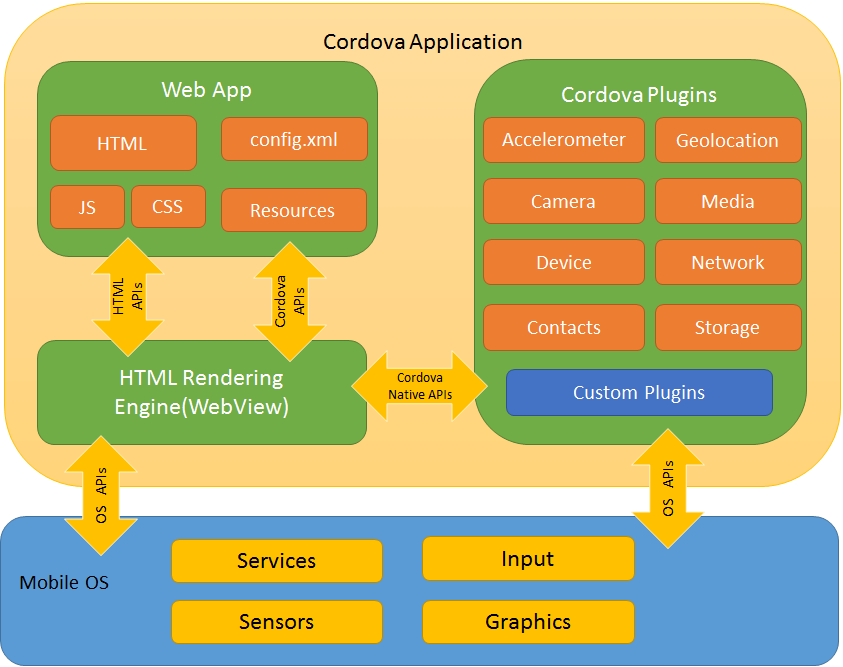
\includegraphics[width=0.6\textwidth]{data/bilder/cordovaapparchitecture.png}
	\caption{Struktureller Aufbau einer Cordova Applikation \cite{cordovaApplicationArchitecture}}
	% https://cordova.apache.org/docs/en/latest/guide/overview/index.html 
	\label{fig:Cordovaapparchitecture}
\end{figure}
%
% --------------------------------------------------------------------------------------------
%
\section{TypeScript}
%
Die von allen modernen Webbrowsern unterstützte Version von JavaScript ist ES5 (ECMAScript 5).
Eine neuere Version von JavaScript, ES6 (ECMAScript 2015), ist eine Obermenge von ES5 was dazu führt, dass ES5-Code stets auch von ES6 unterstützt wird. ES6 wird nicht in vollem Umfang von allen heutigen Browsern unterstützt \cite{compatTableES6}.

TypeScript ist eine von Microsoft entwickelte typisierte Version von ES6, deren Verwendung sich für Ionic 2-Projekte anbietet, da Ionic 2 selbst auch in TypeScript geschrieben ist und so voll typisiert ist \cite{ionic2Docu}.
%https://ionicframework.com/docs/v2/resources/TypeScript/

TypeScript erweitert die Funktioinalitäten von ECMAScript~6 unter anderem um das Konzept fester Datentypen und ermöglicht die Definition eigener Datentypen. Datentypen werden dabei zur Compilezeit überprüft.

Wie aus anderen objektorientierten Programmiersprachen bekannt, verfügen Klassen über das Konzept der Vererbung. Neben Klassen können zudem auch Interfaces definiert werden. Klassen, Interfaces, Funktionen und Variablen können in Modulen in eigenen Namensräumen (\emph{Namespaces}) zusammengefasst werden \cite{MicrosoftTypeScriptDoku}.

Das Konzept der Typisierung von Variablen, den Parametern und Rückgabewerten von Funktionen und die Definition von Interfaces in TypeScript ist in Listing \ref{lst:TypeScriptExample} an einem minimalen Beispiel gezeigt.

\begin{listing}[htb]
    \lstinputlisting{data/sourcecode/typesciptExample.ts}
    \caption{Beispiel zur festen Typisierung in TypeScript}
    \label{lst:TypeScriptExample}
\end{listing}

Wird ein Ionic-Projekt über das Ionic CLI (\enquote{Comand Line Interface}) kompiliert, so findet der sogenannte Transpiling-Vorgang in die vom Browser unterstützte ES5 Version statt. Unter Transpiling, auch source-to-source compiling genannt, wird die Umwandlung von Sourcecode zwischen zwei Programmiersprachen verstanden, die einen ähnlichen Abstraktionslevel besitzen, wohingegen Kompilieren allgemein die Übersetzung von einer Programmiersprache (meist einer high-Level Sprache) in eine andere Sprache (meist eine low-Level Sprache) meint. Transpiling ist also eine spezielle Form des Kompilierens \cite{TranspilingVsCompiling}.
%
% --------------------------------------------------------------------------------------------
%
\section{Angular}
\label{sec:Angular}
%
Angular ist ein von Google entwickeltes clientseitiges JavaScript-Framework zur Erstellung von Single-Page-Webanwendungen. Es arbeitet dabei nach dem Model-View-ViewModel-Entwurfsmuster. Angular baut dabei auf der Erweiterung des Vokabulars von HTML auf und ermöglicht es, Inhalte in der View ohne eine Manipulation des DOM (Document Object Model) anzupassen, ohne selbst JQuery-Manipulationen durchführen zu müssen. Dies geschieht unter Angular mittels Directives.

Die hier betrachtete Version von Angular ist die völlig neugeschriebene Version 2, die auf die Entwicklung mobiler Applikationen ausgelegt ist. Angular 2 ist für die Entwicklung mit der Programmiersprache TypeScript konzipiert. Die finale Version von Angular 2 wurde im September 2016 veröffentlicht.
%
\subsection{Basiskonzepte von Angular 2}
% \cite{DodsonGuideToWebComponents}
% https://css-tricks.com/modular-future-web-components/
Angular 2-Projekte sind in Modulen aufgebaut, die je nach Bedarf mithilfe von imports in andere TypeScript-Dokumente geladen werden können. Als Basiselement werden sogenannte Components verwendet. Components sind wiederverwendbare Komponenten, die einen Teil einer View repräsentieren und dazugehörige Controllerlogik in Form einer TypeScript-Klasse besitzen.

Vor der eigentlichen Klassendefinition werden Components mittels eines decorators eingeleitet, der der Component zusätzliche Informationen wie das zugeordnete Template, das CSS-Style oder den Selector, über den die Component in HTML angesprochen werden kann, liefert. Dieser Mechanismus des Decorators ist in minimaler Form in Listing \ref{lst:decoratorExample} gezeigt.

\begin{listing}[htb]
    \lstinputlisting{data/sourcecode/componentDecoratorExample.ts}
    \caption{Beispiel für einen Decorator einer einfachen Component}
    \label{lst:decoratorExample}
\end{listing}

Innerhalb der TypeScript-Klasse werden Membervariablen und -funktionen bereitgestellt, die aus der View heraus aufgerufen werden können.

HTML5-Templates bilden die View zu einer Component. Mittels Data Binding können die Member der Components mit der View verknüpft werden \cite{LynchAngularComponents}. Data Binding stellt die Datensynchronisation zwischen Model und View dar. Es gibt dabei zwei Arten von Data Binding. One-Way-Data Binding stellt Daten aus dem Model in der View dar. Dies lässt sich in Angular innerhalb der View mittels doppelt geschweiften Klammern realisieren. So werden die im Controller hinterlegten Variablen und Funktionen einseitig mit der View verknüpft. Durch Two-Way-Data Binding mittels der \texttt{ngModel}-Directive lässt sich eine zweiseitige Verknüpfung von View und Model erreichen. Wird die verknüpfte Variable in der View geändert, so wird sie auch im Model angepasst und umgekehrt.

Durch Event Binding werden Elemente einer View mit Angular-Events (z.B. \texttt{focus}, \texttt{blur} und \texttt{click}) oder selbst definierten Events verbunden, die dann Methoden in der jeweiligen Component aufrufen können (vgl. auch  \cite{PrechtAngularTemplateSyntax}).

Angular hat drei Arten von sogenannten Directives: die bereits erwähnten Components, structural Directives und attribute Directives. Directives sind Marker auf einem DOM-Element (z.B. Attribut, Elementname oder CSS-Klasse), die dem Angular HTML-Compiler mitteilen, dass ein bestimmtes Verhalten mit dem jeweiligen DOM-Element verbunden werden soll. Eine Component ist dabei nur eine Spezialform einer Directive mit einem zugeordneten Template.

Mithilfe von \emph{structural Directives} können direkte DOM-Manipulationen vorgenommen werden. So gibt es Angularspezifische Directives wie beispielsweise die  \texttt{*ngFor}-Directive, die wie eine foreach-Schleife einen Container durchlaufen kann und so z.B. schnell eine Tabelle erstellen kann. Ähnlich bedeutend ist die \texttt{*ngIf}-Directive mit deren Hilfe selektiv an eine Bedingung geknüpft Elemente erzeugt werden können.

\emph{Attribute Directives} ändern das Verhalten oder Aussehen bestehender Elemente. So kann beispielsweise mittels der \texttt{ngModel}-Directive ein Two-Way-Data Binding mit einem Attribut einer Component realisiert werden. 

Mittels Referenzen auf einzelne Element des DOM können aus einem Element direkt andere Elemente innerhalb der View angesprochen werden.

Services sind Klassen, die wiederverwendbare Funktionalitäten für Components bereitstellen. Grundsätzlich sollten Components so schlank wie möglich konzipiert sein und die eigentliche Funktionalität sollte in Services ausgelagert werden, um eine wiederverwendbarkeit von Funktionalitäten zu ermöglichen und die Programmlogik übersichtlich zu halten. So sollten Components selbst keine Serveranfragen durchführen oder Daten validieren. Stattdessen sollten solche Aufgaben an Services weitergeleitet werden, die dann in verschiedenen Components Verwendung finden können.
%
Mithilfe des \emph{Dependency injection} Entwurfsmusters \cite{angularDependencyInjectionDoku} werden Components zur Laufzeit mit neuen Instanzen der Services versorgt, die sie benötigen. So werden stets nur die Service-Klassen geladen, die wirklich benötigt werden \cite{angularDocuBasicArchitecture}. Dependency injection findet in Angular 2 über den Konstruktor der Component-Klasse statt. Hier werden die benötigten Abhängigkeiten der Component als Argumente mit übergeben.
%
% --------------------------------------------------------------------------------------------
%
\section{Konzepte des Ionic 2 Frameworks mit Angular 2}
\label{sec:ionicKonzepte}

Das Ionic-Framework liefert eine große Sammlung an Angular 2-Components die sich frei in ein Cordova-Projekt einbauen lassen. Es liefert zudem verschiedene Styles pro Plattform, die durch komplett verschiedene und unabhängige SASS-Dateien realisiert werden. So sorgt Ionic 2 für ein plattformspezifisches Nutzererlebnis. Eine große über 900 Elemente umfassende Sammlung an Icons, die sogenannten Ionicons, passt sich zudem dynamisch dem jeweiligen Betriebssystem an und liefert so ebenfalls einen möglichst passenden Stil, der zur jeweiligen Plattform passt. Ionic Native ist eine Sammlung an TypeScript-Wrappern für Cordova- bzw. PhoneGap-Plugins, also an das Ionic Framework und die Nutzung von Angular zur Erstellung der Webapp angepasste und typisierte Cordova-Plugins, die es ermöglichen grundsätzlich jede Art von nativer Funktionalität zu einer Ionic-App hinzuzufügen \cite{ionic2Docu}.
% https://ionicframework.com/docs/v2/native/

Der große Vorteil in der Verwendung des Ionic-Frameworks ist, dass bereits eine große Zahl an Components vorgefertigt sind, die ansonsten zunächst selbst erstellt und im Style an die jeweilige Plattform einzeln angepasst werden müssten. So liefert Ionic bereits viele für mobile Plattformen typische vorgefertigte Steuerelemente wie Buttons, Listen, Eingabefelder, Checkboxen oder ähnlichen für mobile Geräte typischen Komponenten, die zudem ein den nativen Elementen nachempfundenes Verhalten sowie Styling besitzen. All diese Funktionalitäten lassen sich auch ohne das Ionic Framework realisieren, jedoch wäre dies mit einem sehr großen Mehraufwand verbunden. 

Listing \ref{lst:ionicExampleView} zeigt exemplarisch eine typische View-Implementierung einer Liste (Table-View) mittels der \texttt{ion-list}-, \texttt{ion-item}- und \texttt{ion-thumbnail}-Components. Die Component \texttt{ion-list} erstellt dabei eine Table-View, \texttt{ion-item} liefert eine einzelne Tabellenzeile und \texttt{ion-thumbnail} bietet die Möglichkeit ein kleines Bild in eine Table-View-Zeile einzubinden.

\begin{listing}[htb]
    \lstinputlisting{data/sourcecode/ionicExample.html}
    \caption{Beispiel einer typischen \texttt{ion-list}}
    \label{lst:ionicExampleView}
\end{listing}

Dabei werden mittels der Angular Direktive \texttt{*ngFor} Elemente eines Arrays (hier \enquote{talkers}) aufgelistet. Mittels der in doppelten geschweiften Klammern geschriebenen One-Way-Data Bindings kann auf die Attribute des betrachteten Objektes (hier \enquote{\#talker}) der Schleife zugegriffen werden. Die einzelnen \texttt{ion-item}s werden zudem mit einem Click-Event verknüpft, welches hier eine in der Component implementierten Methode \enquote{\texttt{goToDetailView}} aufruft. Die \texttt{*ngIf}-Bedingung sorgt dafür, dass nur bei erfüllter Bedingung das \texttt{<span>}-Element erzeugt wird.

Listing \ref{lst:ionicExampleTs} zeigt die minimal gehaltene TypeScript-Component zur in Listing \ref{lst:ionicExampleView} dargestellten HTML-View. Ein Interface \texttt{ITalker} definiert den in der View dargestellten Datentyp. Mittels dependency-injection wird ein externer Service namens \texttt{DatabaseService} eingebunden, der im Konstruktor über die Methode des Services \texttt{getTalkersArray} die darzustellenden das Interface \texttt{ITalker} implementierende Objekte in einem Array liefert. Die in der Component definierte Funktion \texttt{goToDetailView}, welche als Parameter ein Objekt vom zuvor definierten Interfacetyp \texttt{ITalker} erwartet, kann über die View aufgerufen werden.

\begin{listing}[htb]
    \lstinputlisting{data/sourcecode/ionicExample.ts}
    \caption{Beispiel einer einfachen Component-Implementation}
    \label{lst:ionicExampleTs}
\end{listing}

Die hier verwendeten Components \texttt{ion-list}, \texttt{ion-item} sowie \texttt{ion-thumbnail} bilden einen sehr komfortablen Weg, auf einfache Art und Weise für mobile Plattformen angepasste Listen zu erstellen. Würde hier auf die Verwendung des Ionic-Frameworks verzichtet müssten diese Components zunächst selbst entwickelt werden.
%
%
% --------------------------------------------------------------------------------------------
% ================================
% = Nicht im Dokument enthalten! =
% ================================
\begin{comment}

\section{Struktur eines Ionic 2-Projektes} 
% https://ionicframework.com/docs/v2/getting-started/tutorial/project-structure/
% http://codingthesmartway.com/ionic-2-project-structure/
\subsection*{./src/}
%
\todo{Soll das Kapitel "Struktur eines Ionic 2-Projektes" raus?}
%
Innerhalb des src-Ordners liegt der unkompillierte TypeScriptcode sowie die Templates. Wird der Buildvorgang per CLI in Gang gesetzt, wird der Code im src-Ordner mittels Transpiling in die korrekte JavaScriptversion umgewandelt und in den www-Ordner kopiert.

Im Unterordner \texttt{./src/app/} wird die Haupt-Komponente der App gespeichert. Diese bildet den Eintrittspunkt der App, das sogenannte \emph{root module} aus dem heraus alle anderen Komponenten geladen werden.

Im Unterordner \texttt{./src/pages/} werden alle weiteren Unterseiten der App mit ihren Komponenten gespeichert. Jede Page besteht dabei aus einem weiteren Unterordner mit grundsätzlich je einer View (.html), einer Komponente (.ts) und der zugehörigen Style-Datei (.scss).
%
\subsection*{./src/index.html}
In der \texttt{index.html} werden benötigte Scripte und Styles geladen und die eigentliche ionic-App wird mit dem \texttt{<ion-app>}-Tag gestartet. Zudem werden die benötigten Skripte \texttt{cordova.js} und \texttt{build/main.js} geladen.
%
\subsection*{./resources/}
Im Ordner \texttt{resources} liegen die für die App nötigen je nach Plattform typischen Icons und Splashscreens (Startbildschirmbilder). 
%
\subsection*{./assets/}
Im Ordner \texttt{assets} werden Ressourcen der App bereitgestellt, die bereits zu Beginn zur Verfügung gestellt werden sollen. So können Datenbanken bereitgestellt werden oder Bilder abgelegt werden.
%
\end{comment}
%\chapter{Unterstützung nativer Komponenten in Ionic}
%
Cordova- und somit auch Ionic-Apps bieten die Möglichkeit um native Funktionalitäten des jeweiligen Betriebssystems mittels Plugins erweitert zu werden.

Ionic bietet eine ganze Reihe von eigenen nativen Komponenten (\emph{Ionic Native}) an, die bereits mitgeliefert werden und nicht extra eingebunden werden müssen. Diese werden lediglich aus der Bibliothek \texttt{ionic-native} importiert.

Ionic bietet zudem einen eigenen Vertriebsmarkt für Plugins an, in dem Entwickler ihre selbst geschriebenen Erweiterungen für Ionic entweder zum kostenfreien download unter einer Open Source Lizenz oder zum kostenpflichtigen Verkauf anbieten können. 

Im Folgenden soll eine sehr spezielle iOS-Funktionalität, nämlich die Unterstützung einer Kommunikation zwischen einer Ionic-App und einer Apple Watch-Anwendung gezeigt werden.
%
\section{Unterstützung von nativen Apple Watch-Apps}
%
Im April 2015 hat Apple die Smart Watch Apple Watch veröffentlicht, die mit sogenannten WatchKit Apps erweitert werden kann. WatchKit Apps gehören jeweils zu einer iOS iPhone-App und werden gemeinsam mit dem App-Bundle der iOS-App ausgeliefert \cite{appleAppleWatchProgrammingGuide}. Apple Watch Apps lassen sich zum jetzigen Zeitpunkt nicht mit Cordova realisieren, da sich innerhalb von Watchkit Apps keine Webviews darstellen lassen. Somit ist eine Schnittstelle, wie sie für hybride Apps erforderlich ist, nicht möglich.

Zur Anbindung einer Apple Watch App an eine Cordova-App gibt es ein passendes Open Source Plugin \cite{CrossleyCordovaAppleWatchPlugin}, dessen Verwendung im Folgenden kurz erklärt wird.

Das Plugin liefert drei Arten der Kommunikation zwischen iPhone und Apple Watch:
\begin{itemize}
    \item \emph{Message passing:} Zweiseitige Übertragung von Strings oder JSON-Objekten zwischen Apple Watch- und Cordova-App.
    \item \emph{Local notifications:} Direktes Senden von Benachrichtigungen aus einer Cordova-App an die Apple Watch.
    \item \emph{User defaults:} Speichern von Daten, die sowohl von der Cordova- als auch von der Apple Watch-App zugänglich sind.
\end{itemize}
%
Der grundlegende Aufbau der Kommunikation zwischen Cordova- und Apple Watch-App ist in \fref{fig:watchPlugin} dargestellt. Das Plugin kommuniziert dabei mit einer iOS-Bibliothek namens MMWormhole \cite{gitMMWormhole}.
% https://github.com/20steps/cordova-plugin-watch
% https://github.com/mutualmobile/MMWormhole
% https://github.com/leecrossley/cordova-plugin-apple-watch#message-passing
% https://github.com/MobileChromeApps/cordova-plugin-background-app
%
\begin{figure}[!htb] 
	\centering
	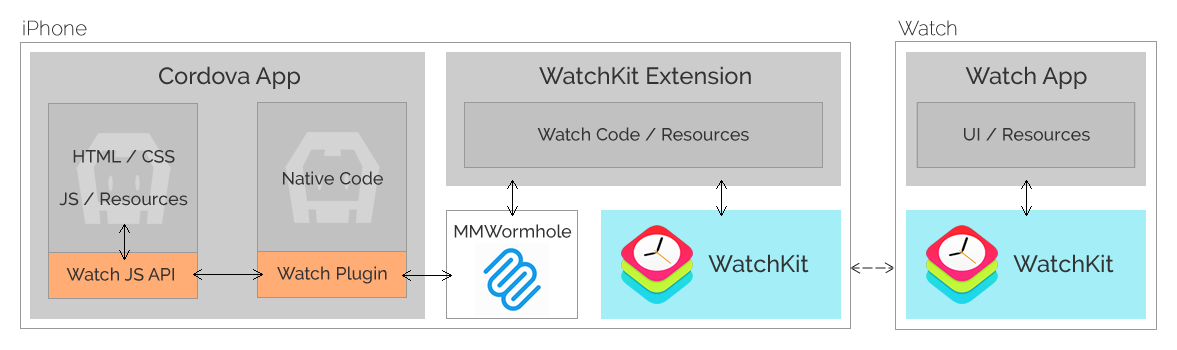
\includegraphics[width=0.9\textwidth]{data/bilder/apple-watch-plugin.png}
	\caption{Prinzip der Nachrichtenübermittlung mittels des Watch-Plugins \cite{CrossleyCordovaAppleWatchPlugin}}
	\label{fig:watchPlugin}
\end{figure}
%
MMWormhole erstellt dabei eine Brücke zwischen der App und ihrer Erweiterung mithilfe von \emph{App Groups}, die die iOS-Plattform seit Version 8 unterstützt. App Groups bieten mehreren Applikationen eines Entwicklers die Möglichkeit auf gemeinsame Daten zuzugreifen. So können auch Daten zwischen einer Extension und der eigentlichen iOS App ausgetauscht werden, was ansonsten aufgrund des Sandbox-Designs von iOS nicht möglich wäre. Das Watch-Plugin steht also über die vom MMWormhole geschaffene Brücke mit dem gemeinsamen Speicherbereich von Apple Watch- und Ionic-App in einer Verbindung und kann so die bereits erwähnten Austauschmethoden anbieten.
%
% --------------------------------------------------------------------------------------------
%
\subsection{Grundsätzliche Methodik} 
%
Sowohl in der Ionic- als auch in der Watch-App muss innnerhalb von Xcode die Nutzung einer gemeinsamen App Group mit fester Group Id definiert werden. Dies muss auch bei der Ionic-App manuell in Xcode geschehen.
%
\subsubsection{Ionic-Seite}
%
Bevor eine Kommunikation zwischen den beiden Plattformen erfolgen kann muss eine Initialisierung stattfinden. Dazu wird eine Initialisierungsmethode \texttt{applewatch.init} aufgerufen:
\begin{lstlisting}[language=JavaScript]
applewatch.init(successHandler, errorHandler, appGroupId);
\end{lstlisting}
Dabei wird mittels des Parameters \texttt{appGroupId} die Application Group Id übergeben, die in Xcode zuvor festgelegt wurde. Dies führt zur Bindung an die in Xcode festgelegte Application Group.

Die Methode \texttt{sendMessage} ermöglicht es, nach erfolgreicher Initialisierung, Strings oder JSON-Objekte an die Watch App zu senden. JSON-Objekte werden dabei automatisch in Strings umgewandelt. 

\begin{lstlisting}[language=JavaScript]
applewatch.sendMessage(message, queueName, successHandler, errorHandler);
\end{lstlisting}
Der Parameter \texttt{queueName} muss dabei mit dem entsprechenden Listener der Watch App Funktion \texttt{MMWormhole.listenForMessageWithIdentifier} übereinstimmen. 

Mittels Listener-Funktionen auf Cordova-Seite können von der Apple Watch ausgesendete Nachrichten empfangen werden. Auch hier muss \texttt{queueName} mit der entsprechenden Methode auf Apple Watch Seite übereinstimmen.
\begin{lstlisting}[language=JavaScript]
applewatch.addListener(queueName, messageHandler);
applewatch.removeListener(queueName, successHandler, errorHandler);
\end{lstlisting}

Lokale Benachrichtigungen benötigen ebenfalls eine Registrierung und eine Erlaubnis für den Empfang lokaler Nachrichten. Dazu wird die Funktion \texttt{registerNotifications} erfragt:
\begin{lstlisting}[language=JavaScript]
applewatch.registerNotifications(successHandler, errorHandler);
\end{lstlisting}
Wird die Erlaubnis durch den Nutzer erteilt, wird der \texttt{successHandler} mit true aufgerufen. Sonst wird der \texttt{errorHandler} mit false aufgerufen.

Mithilfe der Funktion \texttt{sendNotification} kann nun eine in einem JSON-Objekt (\texttt{payload}) gekapselte Nachricht an die Apple Watch gesendet werden.  
\begin{lstlisting}[language=JavaScript]
applewatch.sendNotification(successHandler, errorHandler, payload);
\end{lstlisting}

\emph{User defaults} werden dazu genutzt, um Nutzerdaten in Form von einzelnen Key-Value-Paaren zwischen der Watch-Extension und der iOS-App auszutauschen. Mithilfe der Funktion \texttt{sendUserDefaults} kann ein solches Key-Value-Paar gespeichert werden:
\begin{lstlisting}[language=JavaScript, breaklines=true]
applewatch.sendUserDefaults(successHandler, errorHandler, 
    { "myKey": "myValue" }, appGroupId);
\end{lstlisting}
Die Funktion \texttt{getUserDefaults} bietet eine entsprechende Lesemöglichkeit:
\begin{lstlisting}[language=JavaScript]
applewatch.getUserDefaults(successHandler, errorHandler, 
    "myKey", appGroupId);
\end{lstlisting}
%
% --------------------------------------------------------------------------------------------
%
\subsubsection{Apple Watch-Seite}
Auf nativer Watchkit Extension Seite (hier beispielhaft in Swift) muss der Nachrichtenaustausch auch zunächst initialisiert werden:
\begin{lstlisting}[language=swift, breaklines=true]
let listeningSession = MMWormholeSession.sharedListeningSession();
listeningSession.activateSessionListening();

let wormhole = MMWormhole(applicationGroupIdentifier: "group.com.yourcompany", optionalDirectory: nil, transitingType: .SessionContext);
\end{lstlisting}

Die Methoden \texttt{passMessageObject} des MMWormhole-Objektes ermöglicht das Senden von Nachrichten. Mit Hilfe der Funktion \texttt{listenForMessageWithIdentifier} des MMWormholeSession-Objektes kann ein Listener erstellt werden:
\begin{lstlisting}[language=swift, breaklines=true]
wormhole.passMessageObject("titleString", identifier: "queueName");

listeningSession.listenForMessageWithIdentifier("queueName", listener: { (messageObject) -> Void in
    if let message: AnyObject = messageObject {
        // Do something
    }
});
\end{lstlisting}

Um auf die user defaults auf Apple Watch-Seite zugreifen bietet das Framework die Klasse \texttt{NSUserDefaults}. Der bidirektionale Zugriff lässt sich wie folgt realisieren:
\begin{lstlisting}[language=swift, breaklines=true]
let userDefaults = NSUserDefaults(suiteName: "group.com.yourcompany")

var myValue: String? {
    userDefaults?.synchronize()
    return userDefaults?.stringForKey("myKey")
}
\end{lstlisting}
%
%\subsubsection{Beschränkung der austauschbaren Datengröße}
Problematisch ist, dass die Größe der Daten, die mithilfe dieses Plugins ausgetauscht werden können von den vom WatchKit-Framework gesetzten Grenzen für Nachrichten und UserDefaults stark limitiert ist. Eine einzelne Nachricht und jeder einzelne Eintrag in die UserDefaults hat eine maximale Größe von 65,5~KB. \cite{appleWatchPayloadMaximumDatatransfer}. Müssten größere Datenmengen ausgetauscht werden ginge dies nicht mit diesem Plugin. Stattdessen müsste ein Plugin entwickelt werden, was tatsächlichen Dateiaustausch ermöglicht, da für Dateiaustausch keine Beschränkung dieser Art existiert.
%
% --------------------------------------------------------------------------------------------
%
\subsection{Skizze einer möglichen Anwendung}
%
Um die hier beschriebene Funktionalität des Nachrichtenaustausches etwas besser zu verdeutlichen wird im Folgenden die Nutzung des Plugins an einem Beispiel beschrieben werden.

Gegeben ist eine App, in der die Inhalte einer Tagung oder Messe dargestellt werden können. Diese App ist vollständig in Ionic geschrieben und liefert bereits einen Mechanismus, um die Daten der Veranstaltung mit einem Server abzugleichen und lokal zu speichern. Als Datenpersistierung wird eine Web SQL Datenbank verwendet. Diese wird mit einem asynchronen objekt-relationalen JavaScript Mapper namens \emph{persistenceJS} gekapselt, der auf dem Cordova SQLite Plugin aufbaut \cite{persistenceJSDoku}. In der Tagungsapp werden unter anderem Listen von Vorträgen und Diskussionsbeiträgen mit ihren Detailinformationen dargestellt. Nutzer können dabei einzelne Beiträge als Favoriten markieren. Zudem können sich einzelne Teilnehmer mit anderen Teilnehmern und Ausstellern verabreden und Termine verabreden, die anschließend in einem App-eigenen Kalender dargestellt werden.

In einer möglichen zugehörigen Apple Watch Companion-App sollen ausgewählte Inhalte wie favorisierte Vorträge oder die Terminabsprachen auf der Watch-App aufgeführt werden. Die Apple Watch-App zeigt also einen sehr kleinen, ausgewählten Teil der Daten der Ionic-App in angemessener Form. Ein Mockup für eine solche Realisierung ist in \fref{fig:AppleWatchMockup} dargestellt. 

\begin{figure}[htb] 
	\centering
	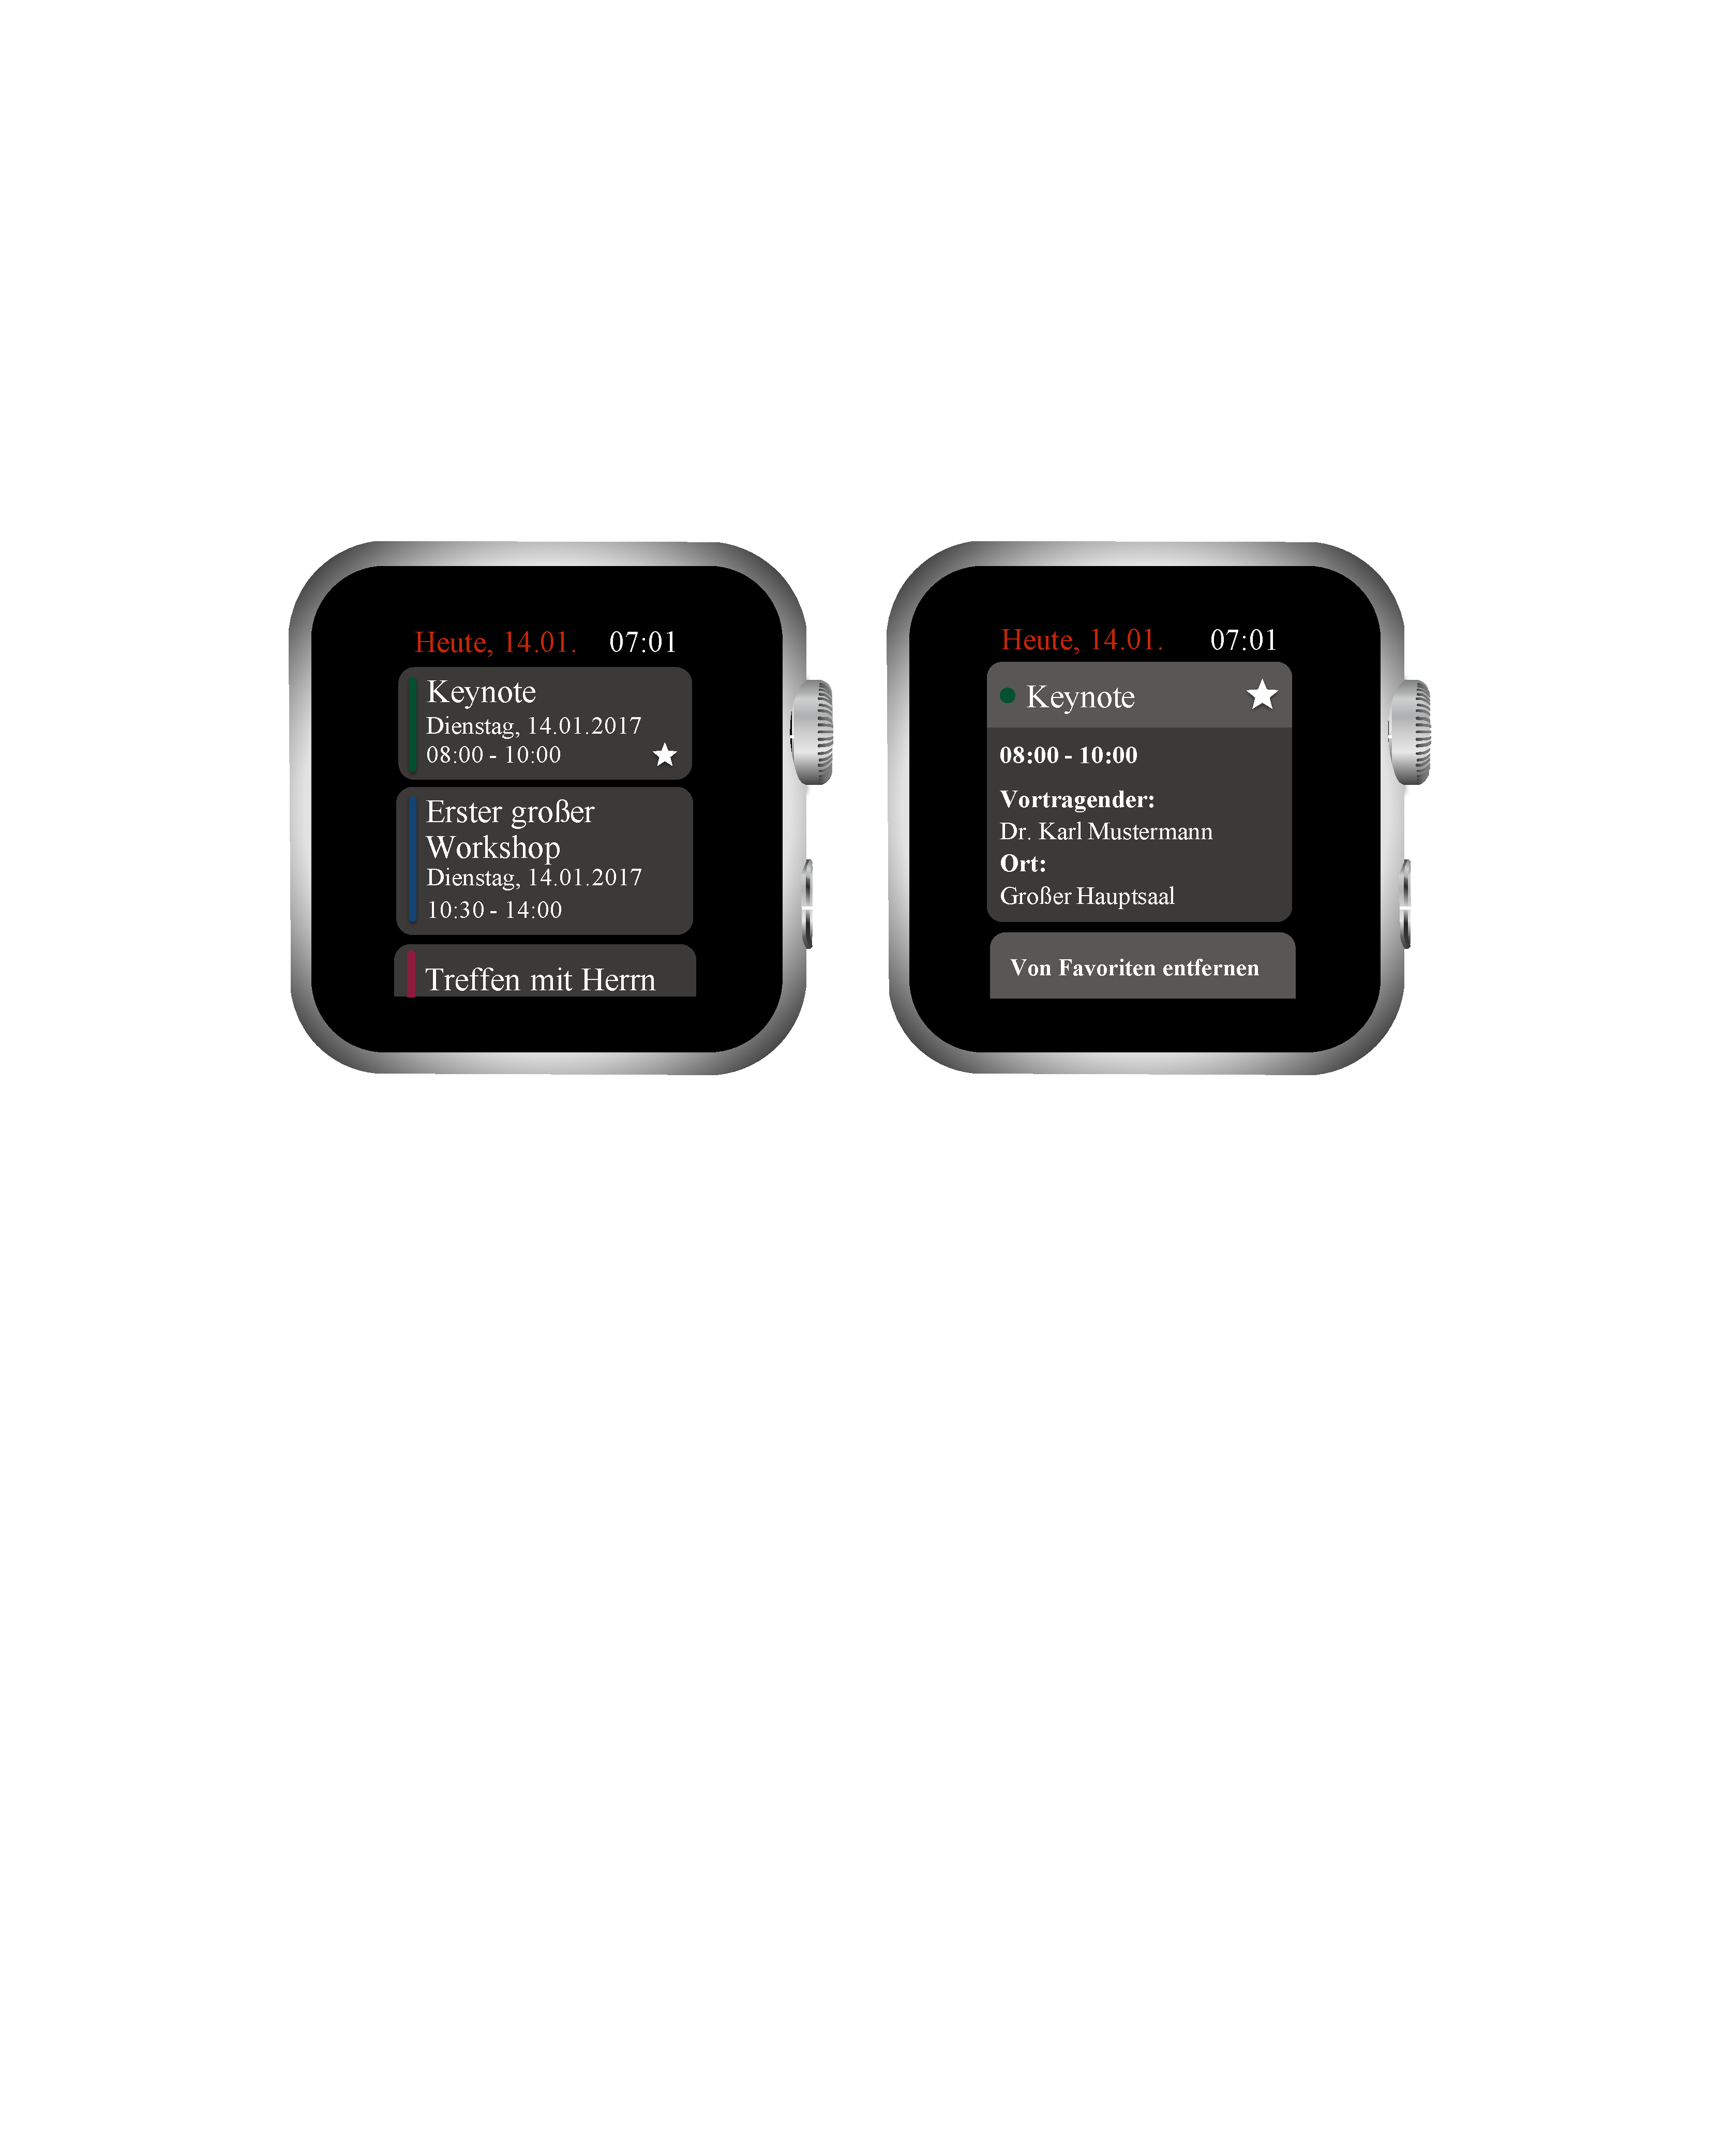
\includegraphics[width=0.6\textwidth]{data/bilder/AppleWatchMockup.pdf}
	\caption{Mockup einer möglichen Realisierung der Datenrepräsentation in einer Table View der Apple Watch und einer möglichen Detailansicht}
	\label{fig:AppleWatchMockup}
\end{figure}

Bei der Konzeption der Apple Watch-App ist darauf zu achten, dass die Smartwatch nur über einen sehr beschränkten Darstellungsbereich verfügt und somit Daten, die auf der Uhr dargestellt werden sollen, auf die wichtigsten Inhalte beschränkt werden müssen. Zudem ist die Eingabe nur über das kleine Display und die \enquote{Digital Crown} sowie den Knopf an der rechten Seite möglich. Apple hat dazu ein eigenes Dokument bereitgestellt, die watchOS Human Interface Guidelines, welche Konzeptprinzipien für gut bedienbare Watch-Apps zusammenfassen \cite{appleWatchInterfaceGuidelines}.

Die wichtigste Kernfunktionalität ist der Datenaustausch zwischen den beiden Plattformen.
Dieser lässt sich mithilfe des Plugins realisieren. Dazu muss der Datensatz aus der SQLite-Datenbank der Ionic-App auf die Kerndaten, die in der Watch-App dargestellt werden sollen, reduziert werden. Anschließend müssen diese Datensätze in Form von JSON-Objekten umgesetzt werden und als String per Nachricht oder über die User defaults an die Apple Watch sendet. Dabei dürfen jedoch nur die nötigsten Daten an im JSON-Objekt gebündelt werden, da die Größe der übermittelten Daten stark beschränkt ist. Beispielhaft ist dieser Vorgang in Listing \ref{lst:watchCommunicationExample} dargestellt. Dem Codebeispiel liegt zugrunde, dass eine in Xcode definierte \texttt{appGroupId} einzigartig ist und eine und über einen Mechanismus wie globale Variable oder einen entsprechenden Mechanismus global verfügbar gemacht wird. Genauso muss auf eine boolsche Variable \texttt{successfullWatchInit} global zugegriffen werden können. 

\begin{listing}[htb]
    \lstinputlisting{data/sourcecode/watchCodeExample.ts}
    \caption{Exemplarischer Datenaustausch für das Tagungsappbeispiel}
    \label{lst:watchCommunicationExample}
\end{listing}

Innerhalb der Apple Watch API gibt es die Klasse \texttt{NSJSONSerialization}, die genutzt werden kann um JSON-Objekte in \texttt{NSDictionary}-Objekte umzuwandeln und die nötigen Informationen für passende Objective~C- oder Swift-Objekte oder für die Speicherung in einer neuen Datenbankstruktur zu erhalten \cite{appleDokuJSONSerialization}. 

Diese Datensätze können anschließend in nativen Table Views der Apple Watch, wie im Mockup in \fref{fig:AppleWatchMockup} gezeigt, dargestellt werden.


%%
%
%
% - - - - - Fazit - - - - - - - - 
%
%
%
\chapter{Fazit}
\label{ch:Fazit}
\insertMore{Fazit}
% 3 Seiten

\printbibliography[title={Literaturverzeichnis}]
\listoffigures

\end{document}